\section{Results}

As it is shown in this section, our findings are consistent with the literature.
In the examined period, among randomly chosen big corporations, the leverage effect in Germany is much stronger and sometimes the return-variance correlation is even positive in China.
Also, in general, the correlation shifted to the left throughout the crisis and its short term aftermath.

\subsection{Chinese anti-leverage}

Figure~\ref{fig:rhos} summarises all the results by plotting all the posterior densities obtained from the dataset.
Even though not all companies behave the same way, there is a consistent picture in general about the differences between the two countries.
The chart shows that, based on the chosen sample, $\rho$ is really estimated to be larger in China than in Germany, except for the periods containing the crisis, when it was similar.

The claims about China behaving differently are strengthened by figure~\ref{fig:negative-rhos}, which shows the number of companies with a significant leverage or anti-leverage effect.
Interestingly, Germany had the least number of companies with significant leverage effect in the period that just preceded the crisis, which was followed by a steep increase in that number.
Apart from the periods containing the boom phase of the 2007 crisis or touching the European debt crisis, the figure for Germany is quite stable around 6-7.
None of the German stocks had a significantly positive $\rho$.

The picture is much less consistent in China.
Ignoring periods with only one significant value, the leverage effect is only observed under the 2007 crisis with some delay compared to Germany, and only in 3 stocks at most, while anti-leverage is also only present before the crisis.
Still, the companies show some consistency, since there is not period with both leverage and anti-leverage effect being present.

Note that the exact distribution or point estimates of $\rho$ are not of high interest.
On the one hand, it is not the correlation of returns with variance changes but with log variance changes, which makes it more difficult to interpret.
On the other hand, comparison with correlation values obtained from other models in the literature is also not trivial, so across models only the sign and highly extreme values are interesting.

\subsection{Time dependence of leverage}

When time-variability is the question, comparison of $\rho$ estimates using the same model for different datasets can be helpful, and figures~\ref{fig:rhos} and~\ref{fig:negative-rhos} suggest that leverage is not constant, not even its sign.
The charts shows that correlation shifts to the negative direction in the crisis, which claim is consistent with recent literature~\citep{christensen2015impact}.
It seems to hold especially for the Chinese stocks since the German companies are more stably on the negative side throughout the whole time.

Figure~\ref{fig:company-rhos} presents more details by showing how the posterior distribution changed with the rolling window of periods.
Indeed, the bottom half of the chart, the German companies are in general below zero since the crisis, showing a quite consistent picture.
BMW and SAP show a steadily strengthening leverage effect, the others either stagnate or show signs of end of the crisis, if we accept the hypothesis from~\citeauthor{Christensen2015}, since the leverage effect is weakening in their case.

Each of the Chinese companies' show far more hectic time-dependence, but all had the negative extremum of the posteriors in a period containing the first half of 2008, at the strongest impact of the crisis.
However, in my view, the overall picture, being so unstable throughout the whole examined time, questions the reliability of the results from the perspective of~\citeauthor{Christensen2015}.
There might be far more and a lot different factors in play that affect Chinese stocks' leverage effect.

\subsection{Volatility estimations}

The posterior of $\phi$ and of the log variance are presented in figure~\ref{fig:persistence} on a chosen subset of periods and companies that represent the whole dataset.
The prior of $\phi$ is taken to be informative, it reflects the empirical fact of highly autocorrelating volatility, which is supposed to improve on convergence of the MCMC method.
The posterior of $\phi$ mainly depends on its prior and the estimate for $\bm h$, hence if the posterior is significantly different from the prior, that means that there is valuable information in $\bm h$ about $\phi$.

An immediately noticeable phenomenon on figure~\ref{fig:persistence} is that the posterior of $\phi$ varies more for the German firms, or more precisely, throughout the crisis and in its short aftermath the volatility of the German stocks was much more persistent than in the other periods.
At the same time, changes in the persistence of the Chinese companies can not be explained by the crisis periods, and the estimates are more stable and closer to the prior, except for the highly persistent 2010-2012 period of 600016 CH Equity.
One can also spot the differences on the log variance timeline: the time series are close to a constant value plus noise in China, containing little information about persistence, contrary to Germany, where clusters of increasing and decreasing trends can be observed around the crisis.

\begin{figure}[p]
	\vspace*{-3.2cm}
	\centering
	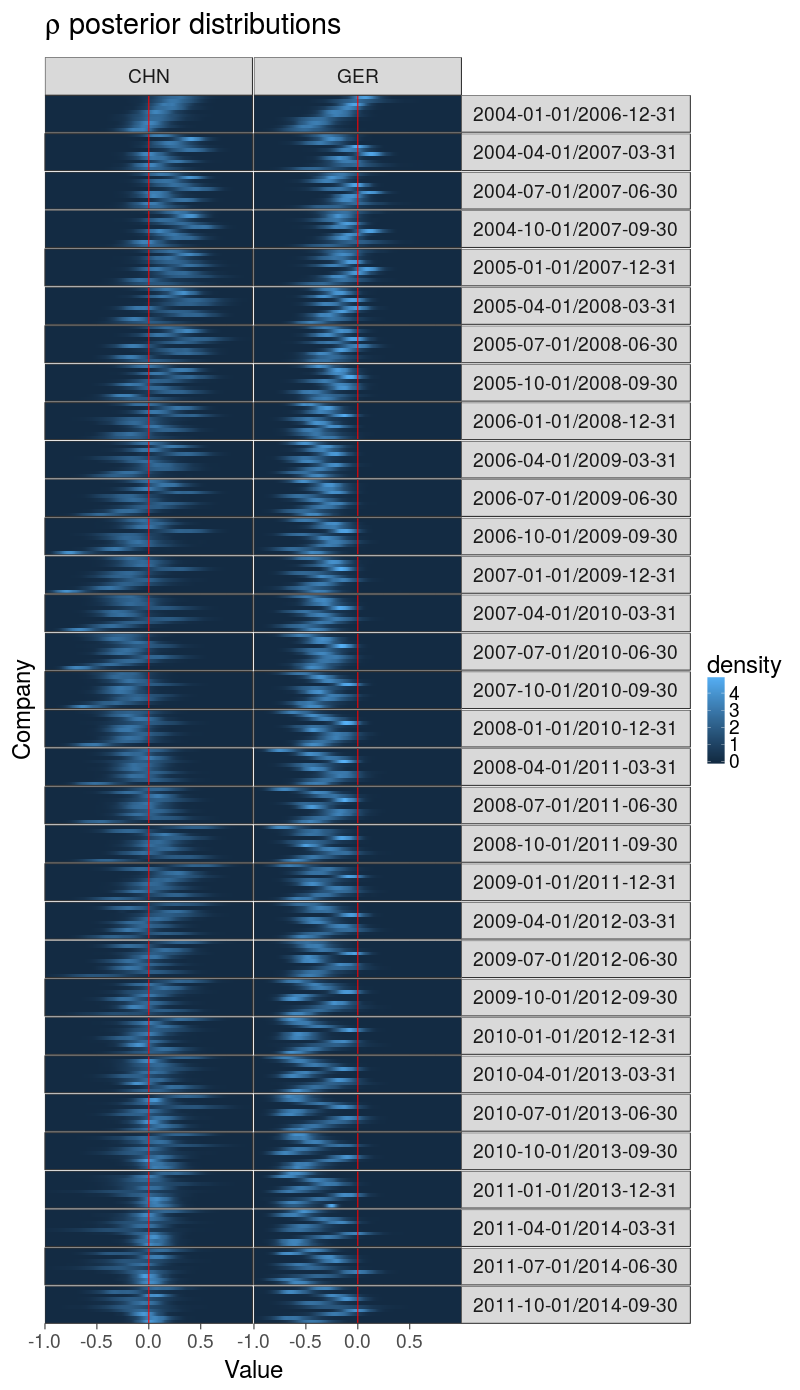
\includegraphics[width=\linewidth]{../calculations/rhos}
	\caption[Visually summarising all results]{Visually summarising all results. Each blue box corresponds to a country and a period and contains 10 rows. One row corresponds to one stock. Each row is a heatmap of $\rho$'s posterior density estimated for that company and period. The red line is constant 0. The stocks' rows are ordered according to their posterior mean in the first period.}
	\label{fig:rhos}
\end{figure}


\begin{figure}[p]
	\vspace*{-3.2cm}
	\centering
	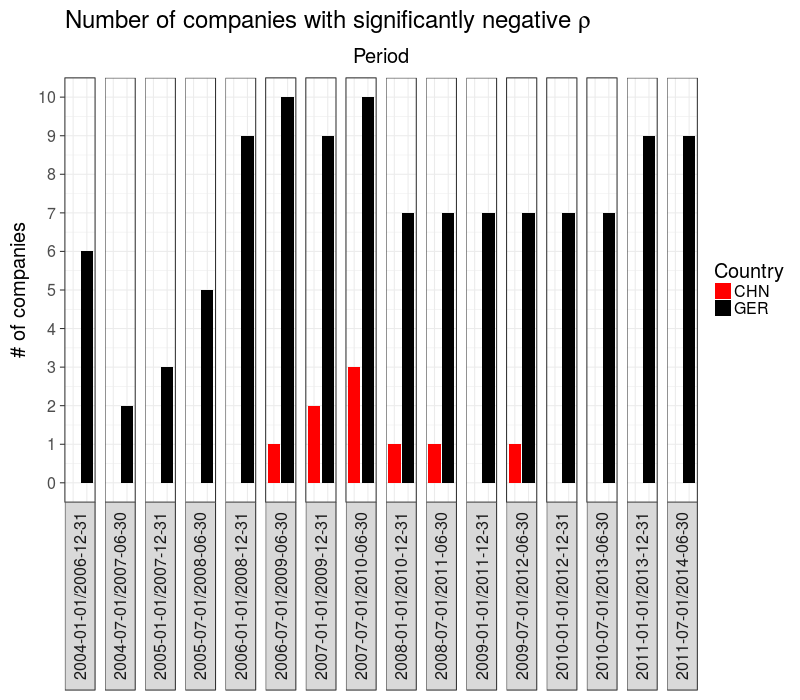
\includegraphics[width=\linewidth]{../calculations/negative-rhos}
	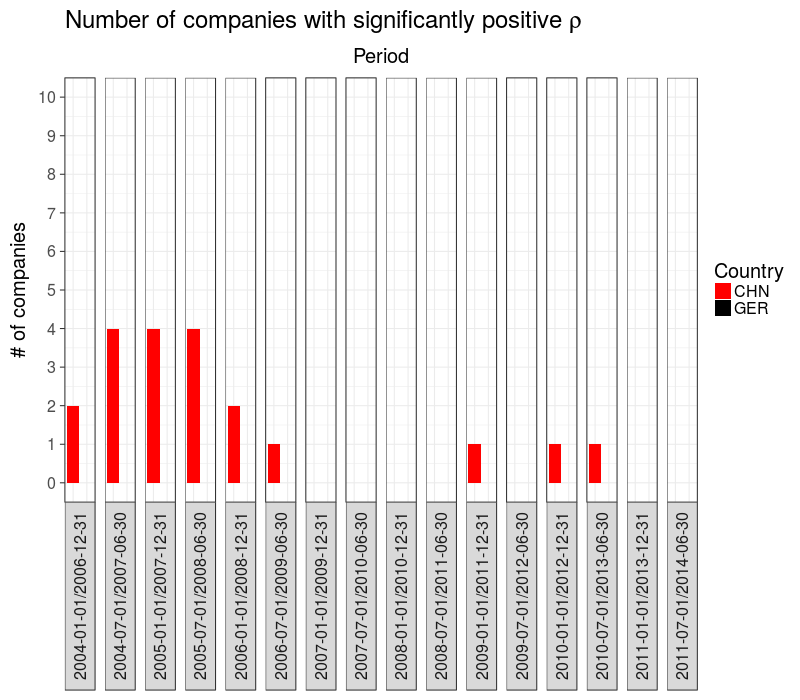
\includegraphics[width=\linewidth]{../calculations/positive-rhos}
	\caption[Significant leverage effect]{Top: number of companies with significant leverage effect per country and period, on a 5\% level. Bottom: number of companies with significant anti-leverage effect per country and period, on a 5\% level. Both: Only every second period is shown for readability.}
	\label{fig:negative-rhos}
\end{figure}


\begin{figure}[p]
	\vspace*{-3.2cm}
	\centering
	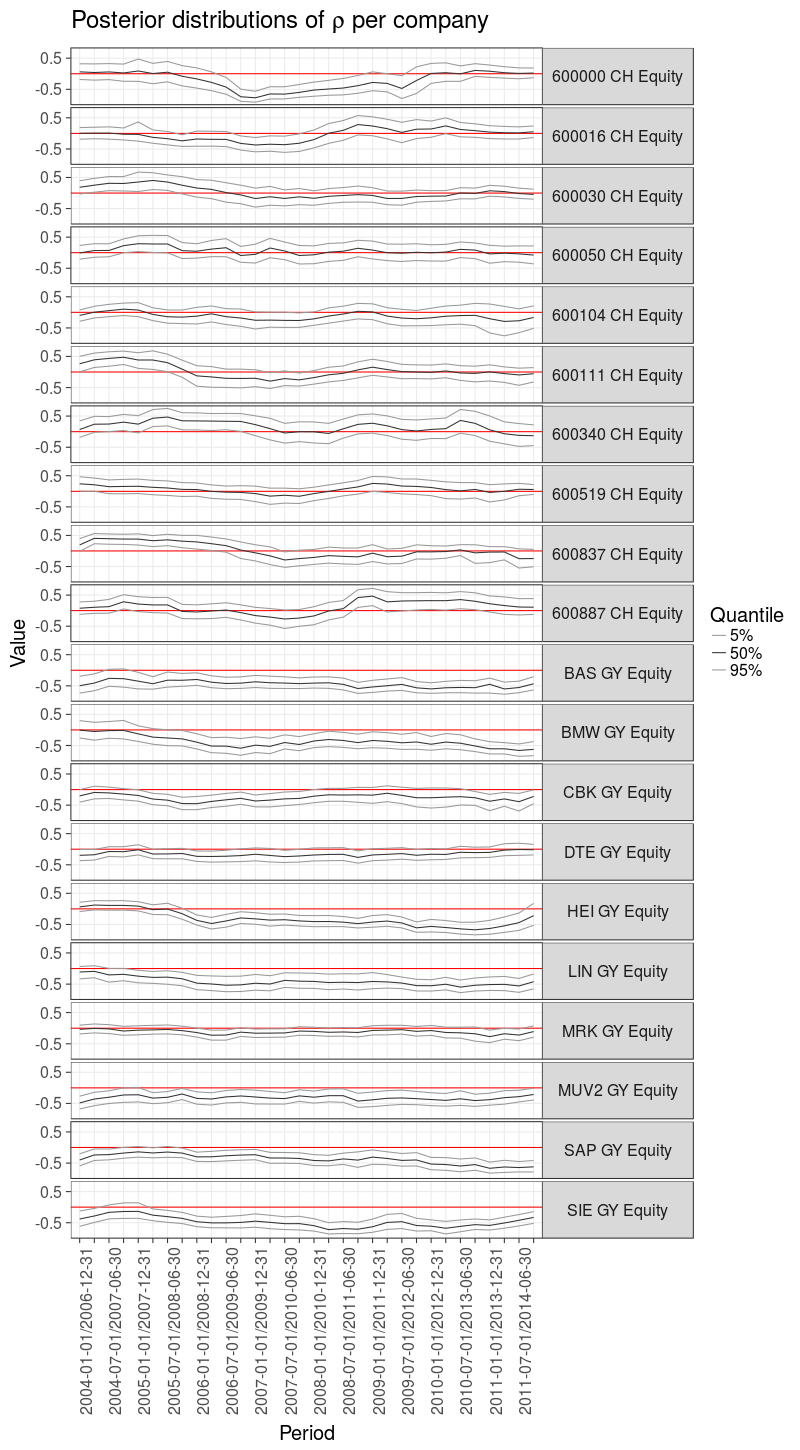
\includegraphics[width=\linewidth]{../calculations/rho-timeline}
	\caption[Timeline of posterior $\rho$]{Posterior distributions of $\rho$ in time. The prior distribution is the standard uniform in all cases.}
	\label{fig:company-rhos}
\end{figure}


\begin{figure}[p]
	\vspace*{-3.2cm}
	\centering
	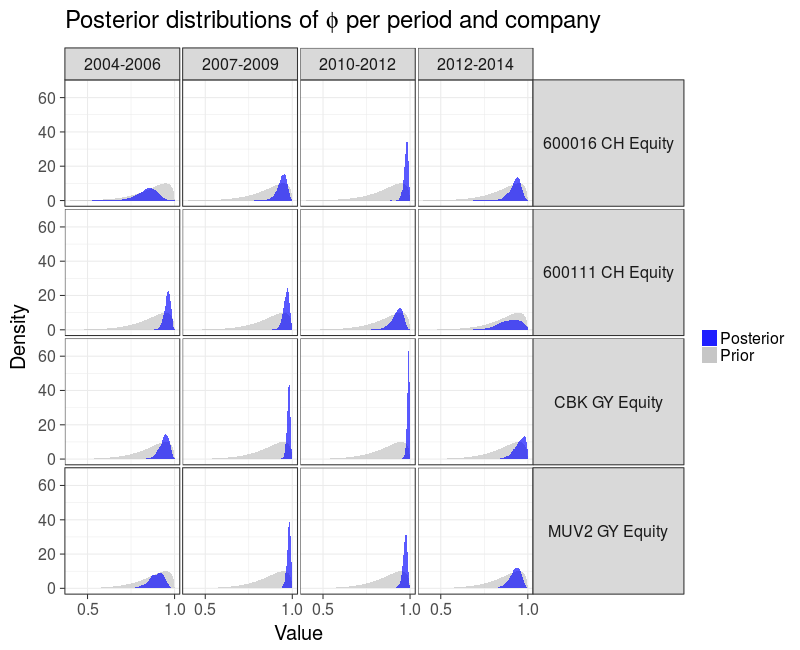
\includegraphics[width=\linewidth]{../calculations/phi-timeline}
	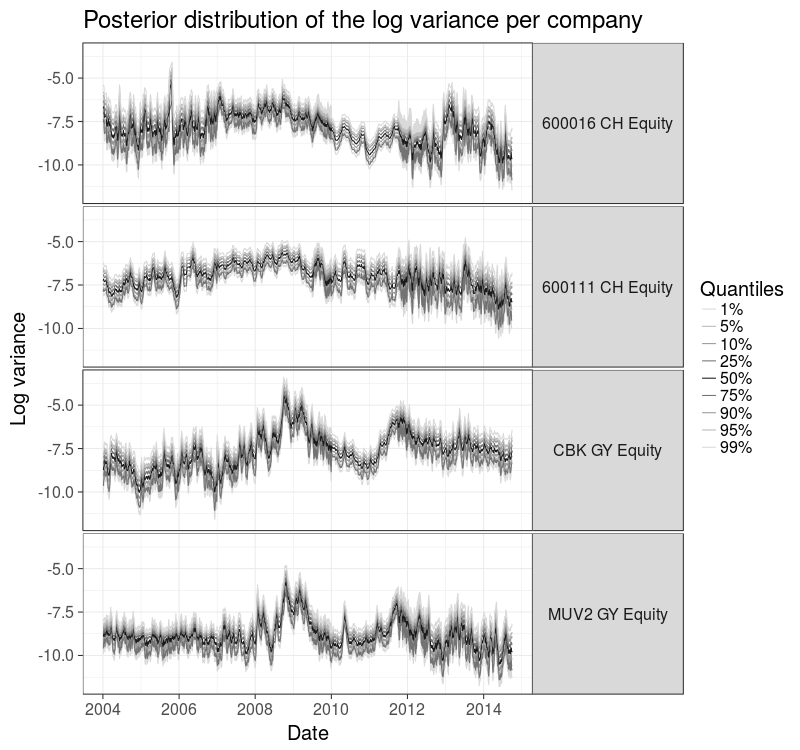
\includegraphics[width=\linewidth]{../calculations/volatility}
	\caption[Timeline of persistence and volatility]{Top: posterior persistence of the log variance for a subset of companies and periods. Bottom: posterior log variance for a subset of the companies. The time series are glued together from the independent volatility estimations from several periods.}
	\label{fig:persistence}
\end{figure}
